\hypertarget{history}{\section{History of community
detection}\label{history}}

Across many disciplines of science, it is common to encounter data that
can best be represented as a network, with entities linked to each other
in some meaningful way, such as through association or flow. These
entities are represented by \emph{nodes} or \emph{vertices} connected to
each other with \emph{links} or \emph{edges}. This overall
representation is known as a \emph{network} or \emph{graph}.\footnote{The
  term \emph{graph} generally refers to a mathematical representation of
  data, while \emph{network} usually has additional connotations related
  to the meaning and context associated with the data
  \autocite{porter_communities_2009}; however, as is the case with many
  terms in this area, the distinction is not always made and the two are
  often used interchangeably.} The idea of community detection as a
research topic comes from a basic intuition that there exist in these
networks groups of nodes that are structurally more related to each
other than they are to members of other groups.

The field of \emph{network science} has emerged recently to study this
and related topics. This field is highly interdisciplinary, comprising
physicists, applied mathematicians, computer scientists, sociologists,
and others. This interdisciplinarity arises both from the variety of
methods that can be applied, and the breadth of potential applications,
often requiring domain-specific knowledge
\autocite{porter_communities_2009}. Within this new field, the concept
of \emph{community} has been somewhat more formalized from the idea
above as a group of nodes (a \emph{subgraph}) with a high concentration
of edges connecting vertices within the group, and a low concentration
of edges with nodes outside the group
\autocite{fortunato_community_2010}.

The earliest analyses of communities were made by social scientists in
the early- to mid-twentieth century---for example Weiss and Jacobson's
analysis of the organizational structure of a government agency
\autocite{weiss_method_1955}. More developments were made by computer
scientists, who began developing graph partitioning algorithms in the
early 1970s to apply to problems in parallel computing and circuit
layout. In 2002, a seminal paper by Girvan and Newman
\autocite{girvan_community_2002} marked the entrance of the physics
community, and ushered in the modern age of community detection
\autocite{lancichinetti_community_2009}. The Girvan and Newman algorithm
introduced in their paper involved successively calculating the
\emph{edge betweenness}---the number of shortest path between all nodes
that run along the edge---of all edges, then removing the edge with the
highest betweenness and repeating. The idea is that the edges with the
highest betweenness centralities are the ones that connect communities,
and the communities can be separated by this divisive algorithm. This
work inspired the development of modularity as a quality measure (see
section on \protect\hyperlink{clustering-perspective}{the clustering
perspective} below). Since then, the field has seen rapid growth and the
development of many new methods.

\hypertarget{community-detection-methods}{\section{Community detection
methods}\label{community-detection-methods}}

\protect\hyperlink{community-detection-methods}{}

What follows is an overview of some of the many community detection
methods currently in use. The overview follows the taxonomy laid out in
a recent paper by Schaub et al. \autocite{schaub_many_2017}. The authors
identify four different perspectives on the problem of community
detection: (i) \protect\hyperlink{the-cut-based-perspective}{the
\emph{cut-based perspective}}, (ii)
\protect\hyperlink{the-clustering-perspective}{the \emph{(data)
clustering perspective}}, (iii)
\protect\hyperlink{the-stochastic-equivalence-perspective}{the
\emph{stochastic equivalence perspective}}, and (iv)
\protect\hyperlink{the-dynamical-perspective}{the \emph{dynamical
perspective}}. The different perspectives represent different approaches
to the problem, often with different kinds of data, different methods,
and different goals. They also represent, to some degree, the different
research communities that have been working on the problem.

\TODO{Add a note about how this might not be the only way to classify the problem space, but it is one way. It does not divide the methods cleanly, but neither do other classification. This is maybe because there are so many connections between methods. Link to discussion in the evaluation section on the need for splitting the problem up.}

\hypertarget{the-cut-based-perspective}{\subsection{The cut-based
perspective}\label{the-cut-based-perspective}}

Some of the earliest work in community detection was in the area of
circuit layout and design. A circuit can be represented as a graph
describing the signal flows between its components. The efficient layout
of of a circuit depends on partitioning the circuit into a fixed number
of similarly sized groups with a small number of edges between
groups---these inter-group edges are known as the \emph{cut}. Similar
problems can be found in load scheduling and parallel computing, where
tasks must be divided into different portions with minimal dependencies
between them. These need for these methods led to the development of the
Kernighan-Lin algorithm in 1970 \autocite{kernighan_efficient_1970},
which has become a classical method that is still frequently used. It
starts with an initial partition and attempts to optimize a quality
function \(Q\) representing the difference between intra-cluster edges
and inter-cluster edges, by swapping equal-sized subsets of vertices
between groups. The method works best if it starts with a decent initial
partition, so in modern use it is often used to refine partitions
obtained using other methods \autocite{fortunato_community_2010}.

The cut-based perspective has also seen the development of spectral
methods for graph partitioning. The spectrum (eigenvalues) of a graph's
adjacency matrix tend to be related to the connectivity of the graph,
and the associated eigenvectors can be used for both cut-based
partitioning and clustering. These methods typically make use of the
Laplacian matrix \(L\) of a connected graph \(G\): \(L = D - A\) where
\(A\) is the adjacency matrix of \(G\) and \(D\) is the diagonal degree
matrix with \(D_{ii} = \sum_{j}{A_{ij}}\). The \emph{Fiedler vector} is
the second-smallest eigenvector associated with the Laplacian matrix
\(L\); the spectral bisection method uses this vector to quickly
partition a graph into two groups with a low cut size
\autocite{fiedler_algebraic_1973}.

A cut-based measure for the quality of a partition is the
\emph{conductance}. The conductance of a subgraph \(S \in V\) for a
graph \(G(V, E)\) is:
\[\phi(S) = \frac{c(S, V \setminus S)}{\min(k_S, k_{V \setminus S})}\]
where \(c(S, V \setminus S)\) is the cut size of \(S\), and \(k_S\) and
\(k_{V \setminus S}\) are the total degrees of \(S\) and the rest of the
graph, respectively \autocite{schaeffer_graph_2007}. While this measure
was originally used globally to optimize a bisection of a graph, it has
also seen use as a local quality function to find good clusters around
certain nodes; in this way it can also be viewed as part of the
clustering perspective \autocite{schaub_many_2017}. Conductance has its
roots in computer science, and its use in network science appears still
to be especially popular in the computer science community
\autocites{schaeffer_graph_2007}{yang_defining_2015}.

\hypertarget{clustering-perspective}{\subsection{The clustering
perspective}\label{clustering-perspective}}

The clustering perspective comes from the world of data clustering, in
which data points are thought of as having ``distance'' between each
other based on their (dis)similarity, and the goal is to group together
data point that are close to each other. For community detection, this
distance is in relation to the connections between nodes in the network.
This perspective is related to but different from the cut-based
perspective above, which seeks to place divisions among the nodes so as
to form balanced groups with weak connections between groups.

A classical method with this perspective is \emph{hierarchical
clustering}, which when used on graphs yields a hierarchical
partitioning that can be viewed as a dendrogram. The common method uses
an agglomerative approach in which each node starts in its own cluster,
and they are joined together one by one based on some similarity measure
calculated using the graph's adjacency matrix. This approach to
community detection has several weaknesses. It necessarily infers a
hierarchical community structure even if one does not exist; the
hierarchy is not always easy to interpret; it often misclassifies nodes,
especially nodes with only one neighbor, which it tends to put it in its
own cluster; and it does not scale well to large networks
\autocite{fortunato_community_2010}.

The \emph{modularity} is a quality function originally developed as
stopping criterion for the Girvan-Newman algorithm (see
\protect\hyperlink{history}{section on history} above)
\autocites{newman_finding_2004}{newman_modularity_2006}. The algorithm
partitions a graph by successively removing links, but the original
formulation did not have a clear stopping point at which the communities
have been identified. The modularity compares an overall partitioning
against a null model. For a given graph \(G(V, E)\) and partitioning
\(\mathcal{C}\), the modularity is:
\[Q = \frac{1}{2m} \sum_{i,j \in V} \left(A_{ij} - \frac{k_i k_j}{2m}\right) \delta(C_i, C_j)\]
where \(m\) is the total number of edges in \(G\), \(A\) is the
adjacency matrix of \(G\), \(k_i\) is the degree of vertex \(i\), and
\(\delta(C_i, C_j)\) is a function that yields one if vertices \(i\) and
\(j\) are in the same community in \(\mathcal{C}\), zero otherwise. The
term \(k_i k_j / 2m\) represents the standard null model used for
modularity---the configuration model which preserves the degree sequence
of the original graph.

Once modularity was introduced, network researchers, especially those in
the physics community, seized on the idea and began developing
clustering algorithms that aim to maximize it---it has become the most
popular and best known quality function
\autocite{fortunato_community_2010}. Finding the optimal modularity for
a graph is an NP-complete problem; finding the global maximum for
modularity on all but the smallest networks is computationally
infeasible, so algorithms attempt to approximate the global maximum of
modularity in a reasonable amount of time. Algorithms tend to have a
tradeoff between speed and accuracy. Greedy algorithms, such as the
original method of Newman \autocite{newman_fast_2004} and the Louvain
method \autocite{blondel_fast_2008} discussed below in the section on
\protect\hyperlink{the-dynamical-perspective}{the dynamical
perspective}, tend to be fast but inaccurate---they discard much of the
problem space in order to arrive at a solution more quickly. Simulated
annealing techniques improve accuracy at the expense of speed by
introducing stochastic noise to nudge the algorithm away from local
maxima; the standard simulated annealing algorithm for modularity can be
found in \autocite{guimera_functional_2005}. Many other techniques,
including spectral optimization and genetic algorithms, have been
employed in attempts to get accurate solutions quickly---see a summary
in \autocite{fortunato_community_2010}.

Modularity became popular in part because it was one of the first
attempts to formalize the concept of community, including in its
mathematical form the definition of community in relation to a defined
null model. The measure has been shown to have some problems, however,
most notably its resolution limit. Modularity-maximizing techniques have
a lower limit on the size of communities it is able to detect which
depends on the number of links and the interconnectedness of communities
\autocite{fortunato_resolution_2007}. This can be a problem in many
real-world networks, which can contain communities of many different
sizes. In addition, modularity can be very sensitive to even individual
connections, which can be a problem in any noisy dataset which can
contain false positives \autocite{fortunato_community_2010}.

\hypertarget{the-stochastic-equivalence-perspective}{\subsection{The
stochastic equivalence
perspective}\label{the-stochastic-equivalence-perspective}}

The stochastic equivalence perspective groups nodes by their
connectivity profile---their probability to connect to nodes in other
groups. The most famous model to come from this perspective is the
\emph{stochastic block model} (SBM), a probabilistic generative model
with roots in statistics and social network analysis. The model sees the
community assignment \(g_i\) for each vertex \(i\) as a latent variable,
with nodes in each group having equal probability of connecting to nodes
in any other given group (or to other nodes in the same group). These
probabilities form what is called the \emph{stochastic block matrix} (or
affinity matrix), a \(q \times q\) matrix, \(q\) being the number of
groups, with diagonal elements \(p_{kk}\) being the probabilities that
nodes of block \(k\) are neighbors, and the off-diagonal elements
\(p_{lm}\) being the edge probabilities between different blocks \(l\)
and \(m\). The model is then fit to the data by estimating the
parameters that give the highest likelihood
\autocites{fortunato_community_2016}{schaub_many_2017}. This view of
equivalence between nodes is not bound by definitions of community that
describe the relative density of edges within and across groups, so
these models can capture a broader range of structure than the
previously described techniques; for example, if the diagonal of the
affinity matrix \(p_{kk} = 0, \forall k\), the model describes a
multipartite graph, in which members of a given group can only link to
members of a different group.

There are several advantages to using a generative model such as the SBM
to describe the community structure of a network. A generative model
views the observed data as one realization of an ensemble of possible
networks generated by a stochastic process. Thus, it allows us to make
statistical claims about the network data and its properties, such as
calculating \(p\)-values and confidence intervals for node properties.
By generating new instances of the model, we are also able to speculate
about possible noise in the data, including predicting missing links.

\TODO{disadvantages: see hric 2016 sec 4.10. SBMs are slow and not necessarily possible for very large networks. how to determine the number of clusters is an open problem, although it seems to be solvable}

\hypertarget{the-dynamical-perspective}{\subsection{The dynamical
perspective}\label{the-dynamical-perspective}}

The fourth perspective that Schaub et al. identify is the dynamical
perspective, and it differs from the above three in that it is not
directly concerned with the structure of the network, but rather the
dynamical processes acting on the network. In other words, it aims to
find coarse-grained, simplified representations of the \emph{behavior}
of a system, rather than its topology. Since the structure of a network
has a strong influence on its behavior, the results of these methods can
actually be very related to the above methods. For example, when
modeling the network dynamics using a random walk, the random walker
tends to get ``stuck'' in communities that look very similar to those
identified using \protect\hyperlink{clustering-perspective}{the
clustering perspective}, e.g., modularity. So a modular description of
the random walker's behavior will closely resemble modularity methods'
clustering of the network topology.

The \emph{map equation} uses elements of information theory to describe
a random walker's movements on a network. It does this by quantifying
the amount of information (in bits) it takes to describe the walker's
movements given a particular modular structure of the nodes. The goal is
to exploit the relationship between compression and relevant modular
structure of a system. The optimal compression means that the smallest
number of bits of information is needed to describe the random walker's
movements. The map equation is the minimal description length (MDL) of
the diffusion process modeled by the random walker given a modular
structure.

An analogy can be made to the world of cartography, which is where the
map equation derives its name. Assigning an address to a location in a
city is a way of encoding that location. Parts of an address can be
reused in different locations---there can exist multiple Main Streets in
different cities. Reusing these names makes describing an individual's
movement within a city more efficient (fewer bits), since as long as we
know the individual is staying within the city limits we can just use
street names without causing confusion. The map equation formalizes this
idea mathematically, providing a function that can be optimized to find
good community structure given a network and a model of the dynamics on
that network. The method does not actually find the description of the
network (the codewords that would be used to compress the network), but
rather the lower theoretical limit on the number of bits that would be
needed to do the encoding.

Information theory states that this lower bound for the average length
of a codeword to describe a random variable \(X\) with \(n\) possible
states that occur with frequences \(p_i\) is equal to the entropy of
that random variable: \(H(X) = -\sum_{i=1}^{n}{p_i\log{p_i}}\)
\autocite{cover_elements_2012}. (It is standard to use base-2 for the
logarithms, which yields calculations in bits.) The map equation
imagines that there are separate codebooks for each module (community),
and is thus the combined entropy of each codebook plus an additional
index codebook that allows for switching between modules, rated by their
rates of use:
\[L(\mathsf{M}) = q_{\curvearrowright} H(\mathcal{Q}) + \sum_{i=1}^{m}{p_{\circlearrowright}^{i} H(\mathcal{P}^i)}\]
where \(\mathsf{M}\) is the module partitioning; the left term is the
average length of codewords (entropy) in the index codebook weighted by
the rate of use of the index codebook \(q_{\curvearrowright}\); and the
right term is the average length of codewords in module codebook \(i\)
weighted by the rate of use of this module \(p_{\circlearrowright}\).
This equation can be expanded in terms of the individual node visit
rates; see section ``\protect\hyperlink{pyinfomap}{Infomap
implementation in Python}'' for details.

The node-visit probabilities that define the \(p\)'s and \(q\)'s in the
map equation can be calculated using the PageRank algorithm
\autocite{page_pagerank_1999}, originally developed to rank web pages in
the hyperlinked world wide web. PageRank is essentially eigenvector
centrality---the node-visit probabilities after an infinite random walk
are equal to the leading eigenvector of the adjacency matrix (the
eigenvector associated with the largest eigenvalue). PageRank includes
an additional element: at any step of the random walk, with a given
probability, the walker can ``teleport'' to a random node on the
network. This teleportation is necessary to avoid the possibility of the
random walker getting stuck forever in an area of the network with no
outward links. The random walker represents an ergodic Markov chain---a
time process in which the state at the next step only depends on the
current state, and the probability distribution of all states as time
approaches infinity is well defined.

For undirected networks, this method gives results that are very similar
to \protect\hyperlink{clustering-perspective}{the clustering
perspective} above, since the network structure and first-order dynamics
are so tightly coupled \autocite{schaub_many_2017}. However, for
directed networks, differences can be seen, as the clustering
perspective is more concerned with pair-wise structural relationships
between nodes, while the dynamical perspective deals with directed flow.
This is illustrated in Fig.~\ref{fig:mapvsmod}, in which the difference
between directed links that allow flow between clusters vs.~links that
trap flow within clusters has an effect on the optimal partitioning for
the map equation, but not for modularity.

The map equation approach is flexible and can give different results
given different dynamics induced on the system. For example, instead of
the standard PageRank implementation of the random walker, the
teleportation can be tweaked, e.g., by employing teleportation to links
instead of nodes, or changing the direction of links in strategic
ways---this changes the node visit probabilities used in calculating the
map equation \autocite{lambiotte_ranking_2012}. Another possibility is
the use of higher-order dynamics: instead of modeling the flow as a
first-order Markov process, in which every step of the walker depends
only on the current position, we can take into account the influence of
the position before the current one, or include several time points
before the present. This can have important impacts on the communities
found \autocite{rosvall_memory_2014}.

\begin{figure}
\centering
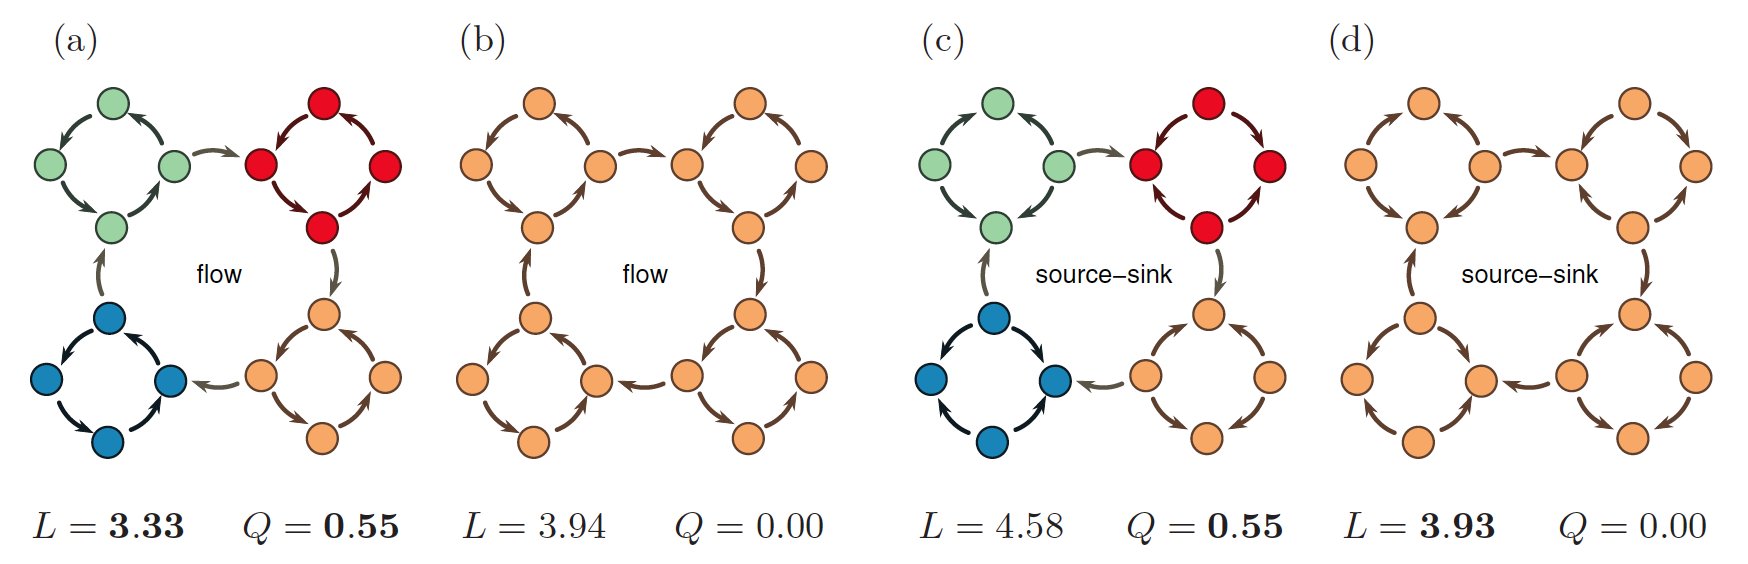
\includegraphics{img/rosvall2010_fig3_mapvsmodularity.png}
\caption{Comparing community detection found using the map equation
vs.~using modularity. For each network diagram, \(L\) is the map
equation, \(Q\) is the modularity, and the colors of the nodes
represents the partitioning. All four networks are the same, except (a)
and (b) have differently directed links than (c) and (d)---the former
allows flow between clusters; the latter traps flow so that the clusters
act as flow sinks. The optimal partitioning---(a) and (c)---are
identical for optimizing modularity, but different for optimizing the
map equation ((a) and (d)). Figure from
\autocite{rosvall_map_2010}}\label{fig:mapvsmod}
\end{figure}

The algorithm used to find the community structure that optimizes is
called Infomap, and the code is available at
\url{http://www.mapequation.org/}. It works similarly to the Louvain
algorithm used to optimize modularity \autocite{blondel_fast_2008}. Each
node starts out in its own module; the modules are joined in a greedy
fashion (examining each node one at a time, in a random order) to yield
the largest increase of the map equation. These modules are joined into
super-modules, the network is reconstructed with these super-modules as
the nodes, and the process is repeated until no further improvement can
be made. This greedy approach has a danger of finding a local optimum,
so at the end, the solution space is further explored by reapplying the
algorithm for each module, and by rerunning the algorithm but allowing
for single-node movements between modules. This method is fast, and so
can be repeated multiple times (with different random seeds) to broaden
the search space more
\autocites{rosvall_maps_2008}{rosvall_map_2010}{rosvall_multilevel_2011}.
See section ``\protect\hyperlink{pyinfomap}{Infomap implementation in
Python} for further discussion on Infomap. The method has been extended
to allow for hierarchical partitions \autocite{rosvall_multilevel_2011},
overlapping communities \autocite{viamontes_esquivel_compression_2011},
and higher-order Markov dynamics \autocite{rosvall_memory_2014}.

\subsection{Future/open problems}\label{futureopen-problems}

\TODO{hierarchical. overlapping.}
